\chapter{Проникновение решетки вихрей в объем жидкости} \label{chapt6}

Как известно \cite{land} волновое движение проникает в глубину жидкости, убывая по экспоненциальному закону:
\begin{equation}
 \label{eq:deepWave}
H(z) = H(0) e^{-kz},
\end{equation}
 где $z$ - глубина, а $k$ - волновой вектор. 
 В предыдущих главах было описано исследование вихревого движения волнами на поверхности жидкости, а так же представлена теоретическая модель, описывающая данное явление.
Согласно построенной модели есть два механизме генерации вихревого движения. 

	Первый, заключается в переносе жидкости в результате дрейфа Стокса. Согласно ему вихревое движение возникает сразу в каждой точке, где появляется волны, и исчезает сразу же как волны затухают или уходят из исследуемой области. Т.е. согласно формулам  (\ref{eq:deepWave}) и (\ref{eq:vortStand}) проникновение вихрей возникающих из-за дрейфа Стокса в глубину должно быть так же экспоненциальным, однако с вдвое большим показателем экспоненты.
\begin{equation}
 \label{eq:deepStocks}
\Omega_{St}(x,y,z) = e^{-2kz} sin \phi H_x(0) H_y(0) \omega k^2 sin(kx)sin(ky)
\end{equation}
Стоит также отметить, что из-за того, что дрейф Стокса наблюдается в лагранжевых координатах, но не в эйлеровых (см. параграф \ref{p1_Stockes}), то это вихревое движение не имеет инерции и не существует отдельно от волн.

	Второй механизм отвечающий за генераций вихрей волновым движение описывает генерацию именно завихренности в эйлеровых координатах. Согласно ему завихренность возникает в результате нелинейного взаимодействия волн в тонком вязком приповерхностной подслое. Для волн частотой 3 Гц на поверхности воды его толщина будет равна $\delta = \sqrt{2 \nu / \omega} \sim 200 $ мкм \cite{FalkovichBook}. Что безусловно мало по сравнению с длиной и даже амплитудой волны, однако больше, чем характерный размер 30 мкм декорирующей частички полиамида PA-12, т.е. частицы полностью увлекаются течением в вязком подслое. Завихренность из вязкого подслоя, проникает в объем диффузионным образом за счет вязкого трения между слоями жидкости. Таким образом, в стационарном режиме предсказывается так же экспоненциальное распределение завихренности по глубине, но отличным от \ref{eq:deepStocks} показателем:
\begin{equation}
 \label{eq:deepEyler}
\Omega_N(x,y,z) = \sqrt{2}e^{-\sqrt{2}kz} sin \phi H_x(0) H_y(0) \omega k^2 sin(kx)sin(ky)
\end{equation}

Для решетки вихрей сгенерированной волновым движение на частота 3 Гц приведенные теоретические оценки (\ref{eq:deepStocks}, \ref{eq:deepEyler}) показывают, что несмотря на то, что размер вихрей составляет половину длины волны $\sim 8$ см, падение амплитуды решетки в $e$ раз стоит ожидать уже на глубине $h = 1/2k \sim 1.4$ см. Исходя из этой оценки был выбран набор глубин, на которых производилось наблюдение за динамикой решетки вихрей: от 0.5 см до 3.5 см.

\section{Экспериментальная методика} \label{sect6_2}
Регистрации завихренности в объеме жидкости производится с помощью методики "лазерного листа". Для декорирования вихревого движения в объем вводятся частички полиамида PA-12, чья плотность близка к плотности воды. Частички подсвечивается лазерным листом, полученным пропусканием лазерного луча через цилиндрическую линзу диаметром 0.6 см, установленную вертикально. В работе использовался лазер MGL-H-532-500mW мощностью 0,5 Вт. После прохождения линзы лазерным лучом, он раскрывался в горизонтальный лазерный лист толщиной около 1 мм. Лазерный лист подсвечивает только те частицы в объеме жидкости, которые встречаются на его пути. Таким образом можно декорировать течения в объеме жидкости лежащие в плоскости лазерного листа. Видеосъемка частиц производилась камерой Canon 70D. Пример получившегося кадра показан на рис \ref{img:track0p5cm}. Однако при волновом движении жидкость колеблется не только в горизонтальной плоскости но и в вертикальном направлении, поэтому декорирующие частички могут входить и выходить из лазерного листа, что приводит к ухудшению точности обработки. Для нивелирования этого эффекта частота съемки синхронизирована с частотой колебаний, т.е. декорирующие частички снимаются при одинаковой фазы волны. Пример поля завихренности показан на рисунке \ref{img:vort0p5cm}.
\begin{figure}[ht]
 \center{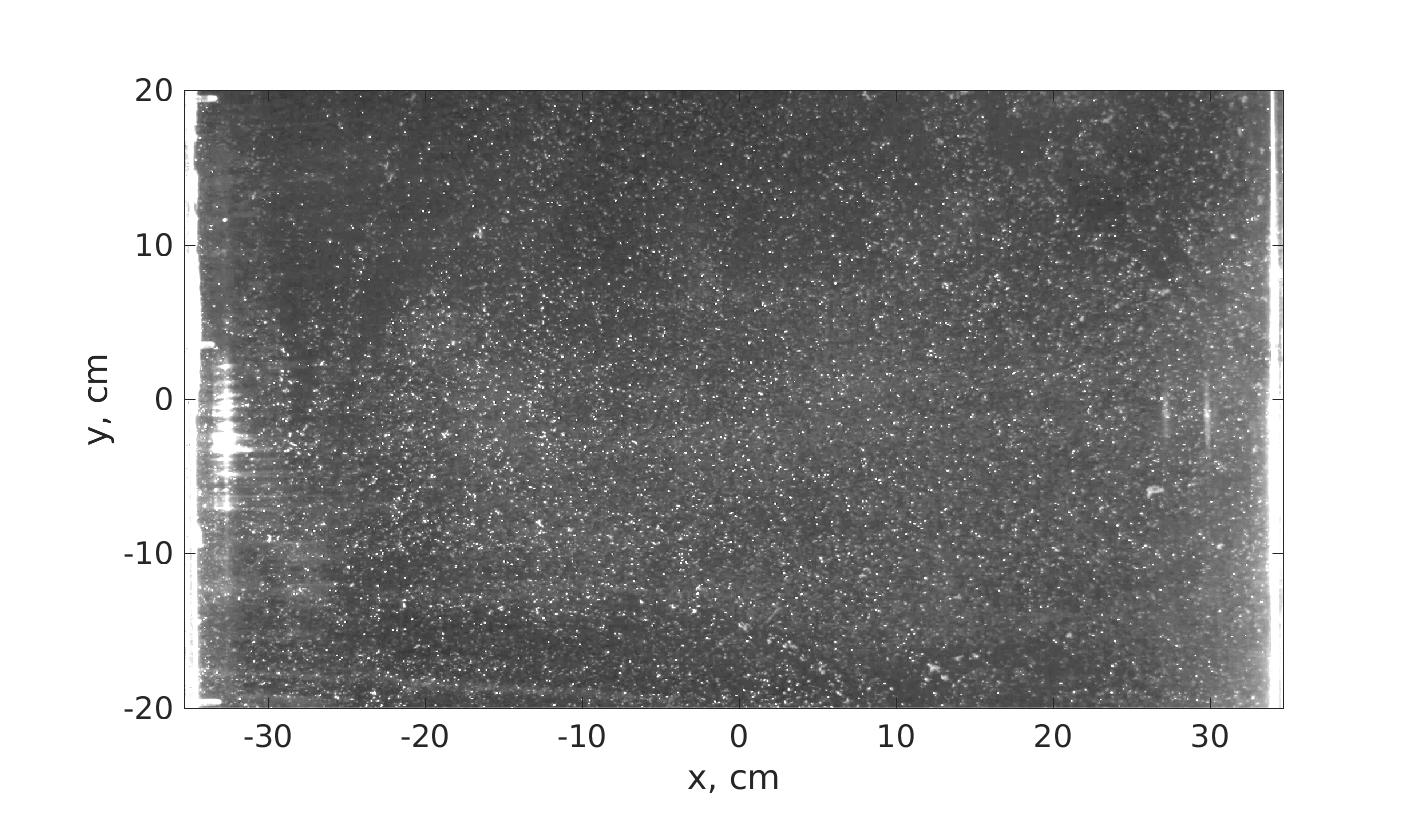
\includegraphics[width=.9\linewidth]{part6/track0p5cm.jpg}}
 \caption{Кадр видеосъемки 40х70 см$^2$ частиц полиамида, подсвеченных лазерным листом в горизонтальном слое на глубине 0.5 см.}
 \label{img:track0p5cm} 
\end{figure}

\begin{figure}[ht]
 \center{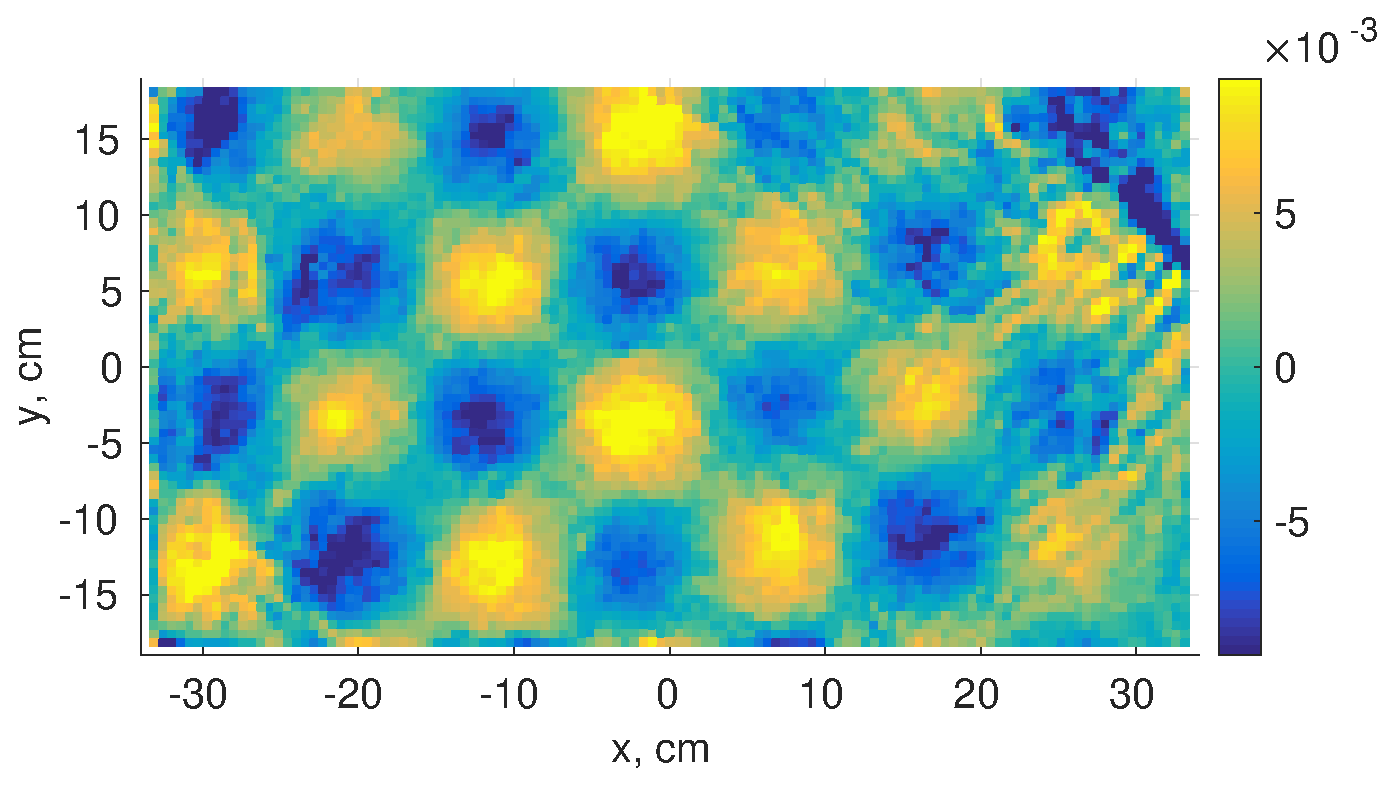
\includegraphics[width=.9\linewidth]{part6/vort0p5cm.eps}}
 \caption{Фрагмент 40х70 см$^2$ поля вертикальной завихренности в горизонтальном слое на глубине 0.5 см.}
 \label{img:vort0p5cm} 
\end{figure}


\section{Экспериментальные результаты} \label{sect6_3}

В эксперименте (рис. \ref{img:5deeps}) было произведено 5 измерений на разных глубинах: 0.5 см, 1.25 см, 2.0 см, 2.75 см, 3.5 см. Накачка производилась на частоте 3 Гц. В каждом измерении записывалась измерение амплитуды завихренности решетки вихрей в течении 600 секунд после включении накачки. На рисунке \ref{img:5deeps} показаны зависимости амплитуд завихренности решетки вихрей от времени для каждой глубины (малой глубине соответствует более высокая кривая на рисунке). Черной кривой показана зависимость $1.4 \cdot 10^{-2} - 8 \cdot 10^{-3} e^{-t/165}$. Видно, что она в среднем хорошо описывает экспериментальную зависимость. Т.е. на глубине 0.5 см завихренность росла с характерным временем 165 с. Оценка характерного времени роста завихренности для других глубин так же дают характерные времена около 200 с. Колебания амплитуды завихренности, которые видны до 200 секунды, связаны с переходными процессами установления волн на поверхности воды после включения накачки (так как накачка производится на частоте немного отличающейся от резонансной частоты системы, то в процессе установления стоячей волн происходят биения с характерной частотой равной разности частот вынуждающей силы и собственных колебаний системы).

\begin{figure}[ht]
 \center{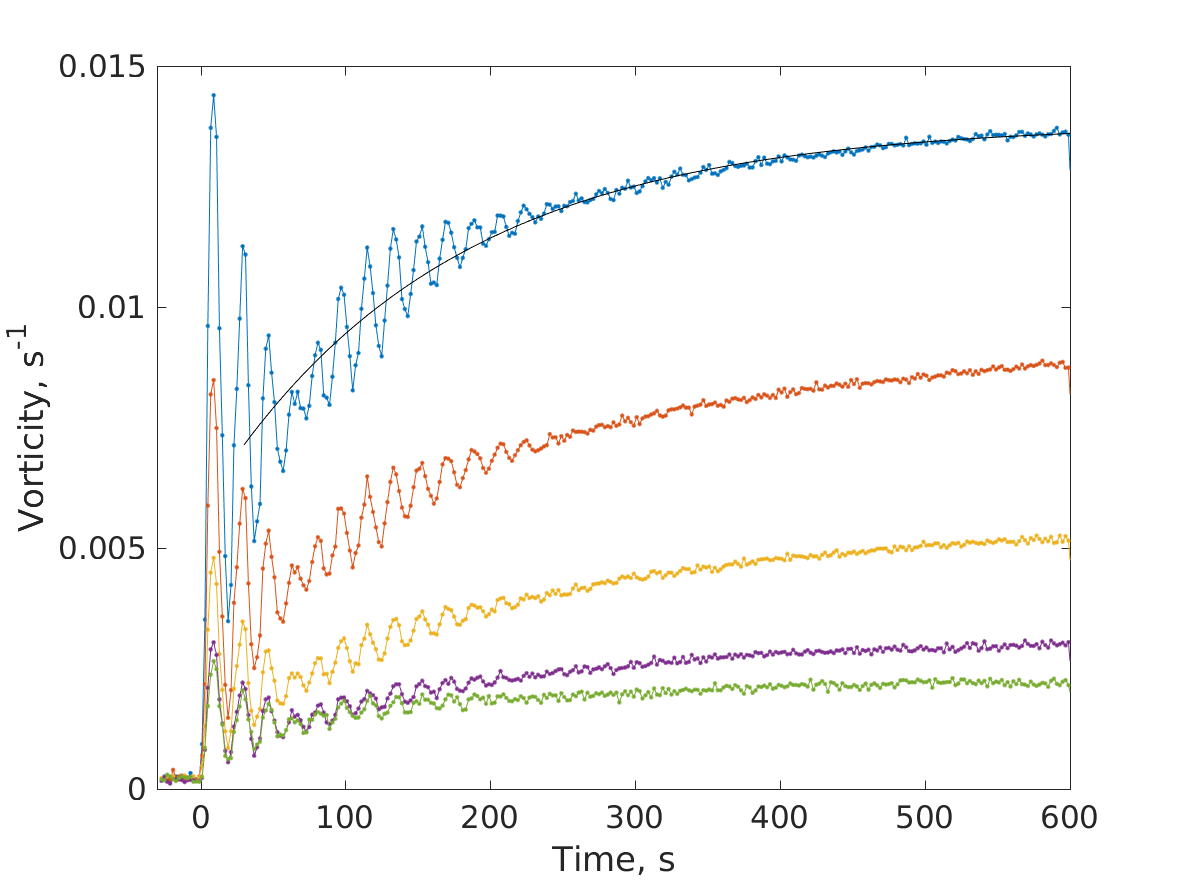
\includegraphics[width=.9\linewidth]{part6/5deeps.jpg}}
 \caption{Зависимость амплитуды завихренности решетки вихрей от времени, на глубинах 0.5 см, 1.25 см, 2.0 см, 2.75 см, 3.5 см. Черная кривая соответствует зависимости $1.4 \cdot 10^{-2} - 8 \cdot 10^{-3} e^{-t/165}$.}
 \label{img:5deeps} 
\end{figure}

Для понимания механизма проникновения структуры вихрей в глубину жидкости рассмотрим Фурье образ поля завихренности на разных глубинах в начальный интервал времени (50-100 секунд после включения накачки) и через 10 минут после включения накачки (550-600 секунды). Соответствующие графики показаны на рисунках \ref{img:detphFFT} а-е. На рисунках видно, что в один и тот же интервал времени структура завихренности на разных глубинах одинаковая. Однако она меняется со временем. Это изменение можно связать с тем, что помимо решетки вихрей в жидкости возбуждаются крупномасштабные вихри, которые сносят решетку завихренности, продиффундировавшую из вязкого подслоя. А снос решетки крупномасштабным течение приводит к искажению квадратной решетки, которое наблюдаются на рис. \ref{img:detphFFT}.

\begin{figure}[ht]
 \begin{minipage}[ht]{0.326\linewidth}
  \center{\includegraphics[width=1\linewidth]{part6/UnderFFT/Under_scan3Hz25mV600s0p50cm_050s.eps} \\ а) t = 50 с, h = 0.5 см}
 \end{minipage}
 \hfill
 \begin{minipage}[ht]{0.326\linewidth}
  \center{\includegraphics[width=1\linewidth]{part6/UnderFFT/Under_scan3Hz25mV600s2p00cm_050s.eps} \\ б) t = 50 с, h = 2.0 см}
 \end{minipage}
 \begin{minipage}[ht]{0.326\linewidth}
  \center{\includegraphics[width=1\linewidth]{part6/UnderFFT/Under_scan3Hz25mV600s3p50cm_050s.eps} \\ в) t = 50 с, h = 3.5 см}
 \end{minipage}
 \begin{minipage}[ht]{0.326\linewidth}
  \center{\includegraphics[width=1\linewidth]{part6/UnderFFT/Under_scan3Hz25mV600s0p50cm_550s.eps} \\ г) t = 550 с, h = 0.5 см}
 \end{minipage}
 \begin{minipage}[ht]{0.326\linewidth}
  \center{\includegraphics[width=1\linewidth]{part6/UnderFFT/Under_scan3Hz25mV600s2p00cm_550s.eps} \\ д) t = 550 с, h = 2.0 см}
 \end{minipage}
 \begin{minipage}[ht]{0.326\linewidth}
  \center{\includegraphics[width=1\linewidth]{part6/UnderFFT/Under_scan3Hz25mV600s3p50cm_550s.eps} \\ е) t = 550 с, h = 3.5 см}
 \end{minipage} 
 \caption{Фурье образ поля завихренности на разных глубинах а-в) в начальный момент времени (50-100 секунд после включения накачки) и г-е) через 10 минут после включения накачки (550-600 секунды).}
 \label{img:detphFFT} 
\end{figure}

Таким образом через некоторое время после включении накачки решетки вихрей искажается. Стоит подчеркнуть, что смещение пиков на фурье спектре показывает именно искажение структуры решетки вихрей, а не полное разрушение. Для оценки количественного влияния крупномасштабных течений на решетку вихрей рассмотрим эволюцию амплитуды решетки вихрей при разных амплитудах накачки (рис. \ref{img:underLong} а-в). На этих же графиках красными кривыми показана временная эволюция скорости крупномасштабных течений  (крупномасштабными будем считать движения с волновым вектором меньшим 0.25 см$^{-1}$). Масштаб для графиков скорости крупномасштабного течения одинаковый на всех трех рисунках. На рисунке \ref{img:underLong} а) видно,что завихренность решетки вихрей растет почти все 1200 секунд, а скорость крупномасштабных течений практически не меняется. В то время на рисунке \ref{img:underLong} б) при большей амплитуде накачки после 400 секунды завихренность решетки вихрей начинает уменьшаться, а скорость крупномасштабных течений растет. Что можно интерпретировать как генерацию крупномасштабных течений, деформирующих решетку вихрей. На рисунке \ref{img:underLong} в) при еще большей амплитуде накачки скорость крупномасштабных течений растет быстрее и завихренность решетки вихрей начинает спадать уже на 200 секунде.

\begin{figure}[ht]
 \begin{minipage}[ht]{0.326\linewidth}
  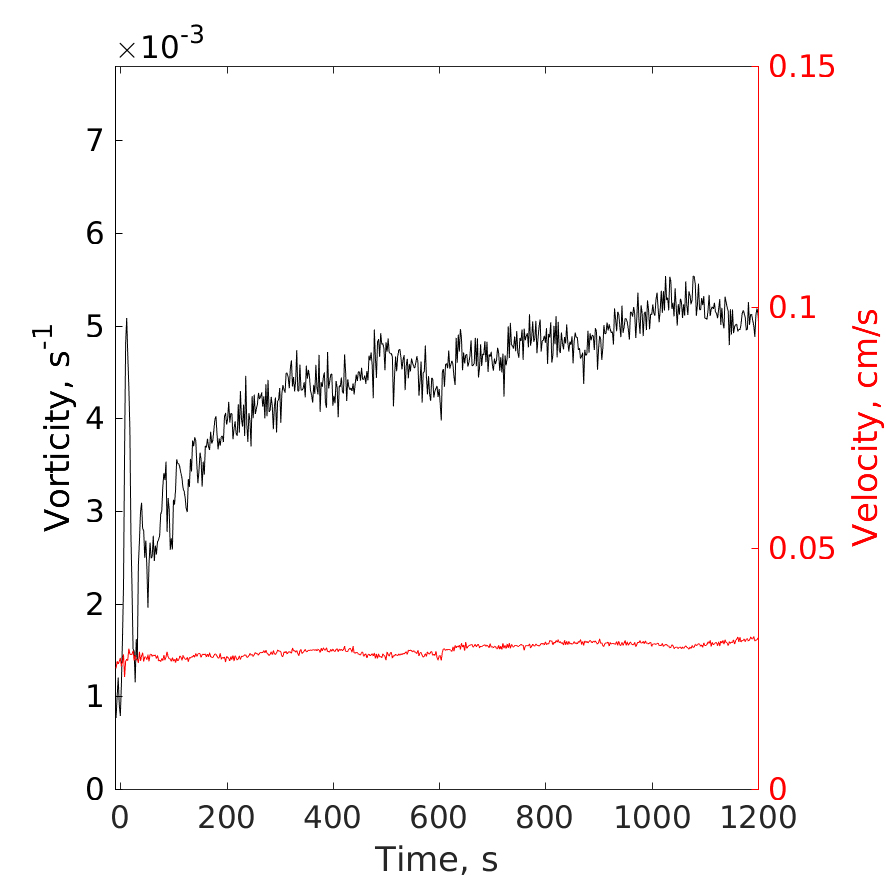
\includegraphics [width=1\linewidth]{part6/long_20mV_vel.jpg} \\ а) 20 мВ, h = 1.0 см
 \end{minipage}
 \begin{minipage}[ht]{0.326\linewidth}
  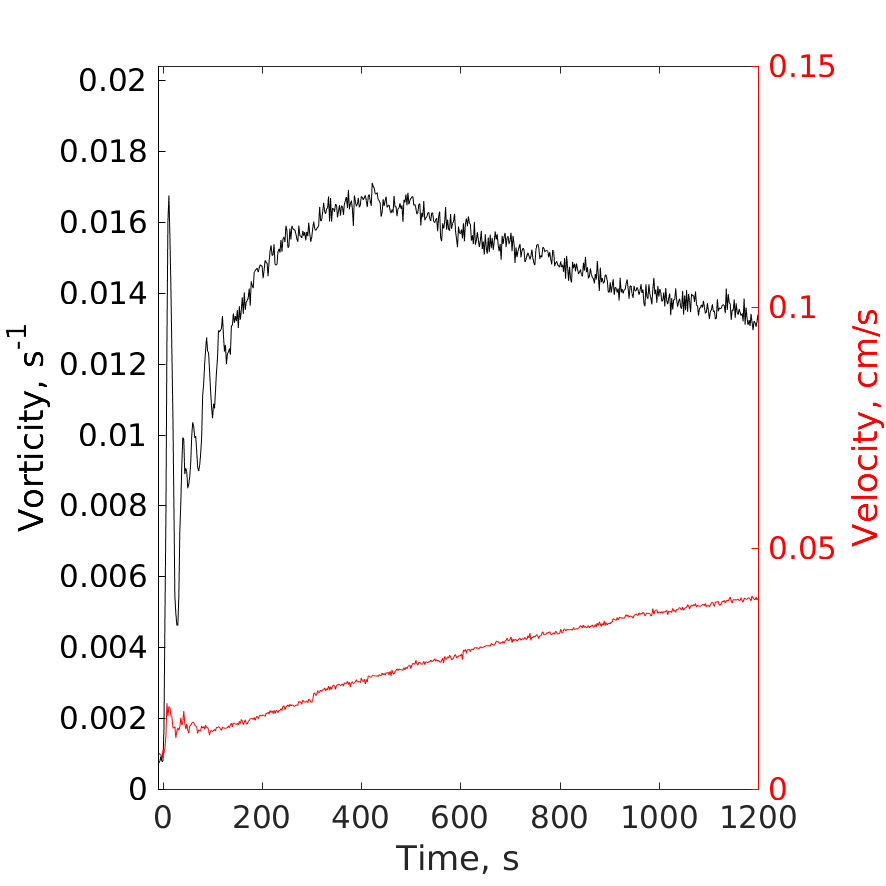
\includegraphics [width=1\linewidth]{part6/long_30mV_vel.jpg} \\ б) 30 мВ, h = 1.0 см
 \end{minipage}
 \begin{minipage}[ht]{0.326\linewidth}
  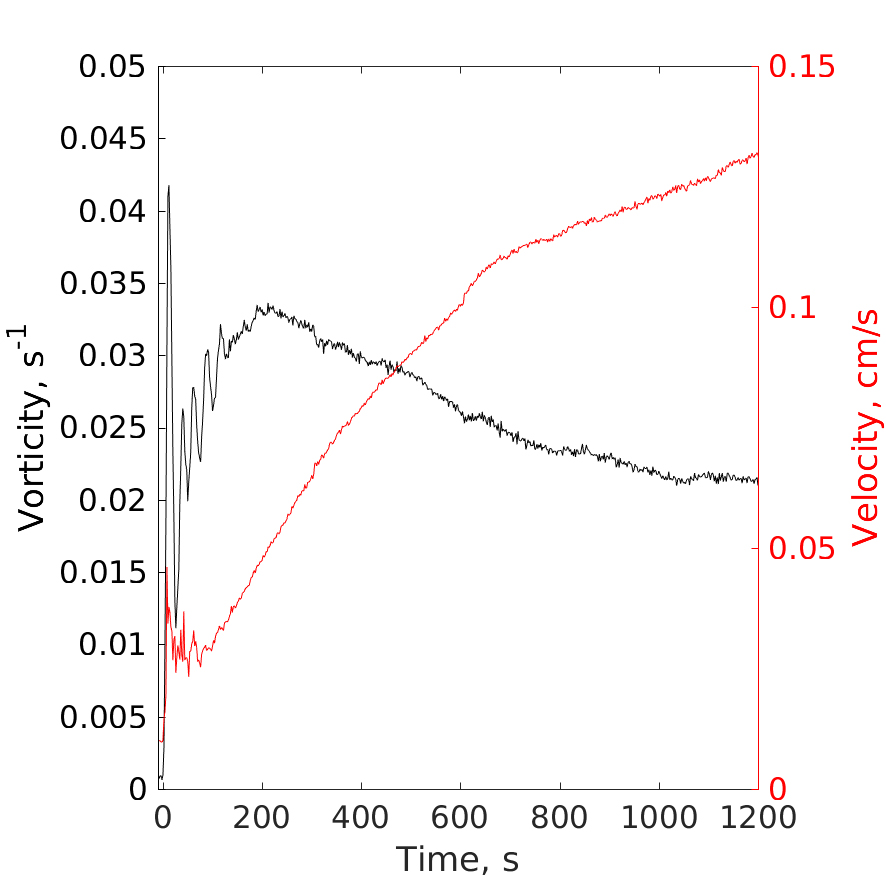
\includegraphics [width=1\linewidth]{part6/long_40mV_vel.jpg} \\ в) 40 мВ, h = 1.0 см
 \end{minipage}
  \caption{Зависимость амплитуды завихренности решетки вихрей и скорости крупномасштабного течения от времени для амплитуд накачки а) 20 мВ, б) 30 мВ, в) 40 мВ на глубине 1 см.}
 \label{img:underLong} 
\end{figure}
\clearpage
\section{Обсуждение экспериментальных результатов} \label{sect6_4}

Из графика \ref{img:5deeps} видно, что характерное время возникновения завихренности в объеме составляет около 200 секунд. Однако из этого же графика видно, что первые 200 секунд происходят колебания завихренности решетки вихрей, что приводит в необходимости понимать как происходит установление волнового процесса на поверхности воды. Для этого на рисунке \ref{img:amplVx} показана зависимость амплитуды горизонтальных колебаний воды от времени (при волновом движении происходит как вертикальные колебания, так и горизонтальные. Измерив скорости $V_x$ и $V_y$ можно получить амплитуду колебательных движений в волне). На экспериментальной зависимости видно, что амплитуда волны первые несколько минут колеблется относительно некого среднего положения.

\begin{figure}[ht]
  \center
  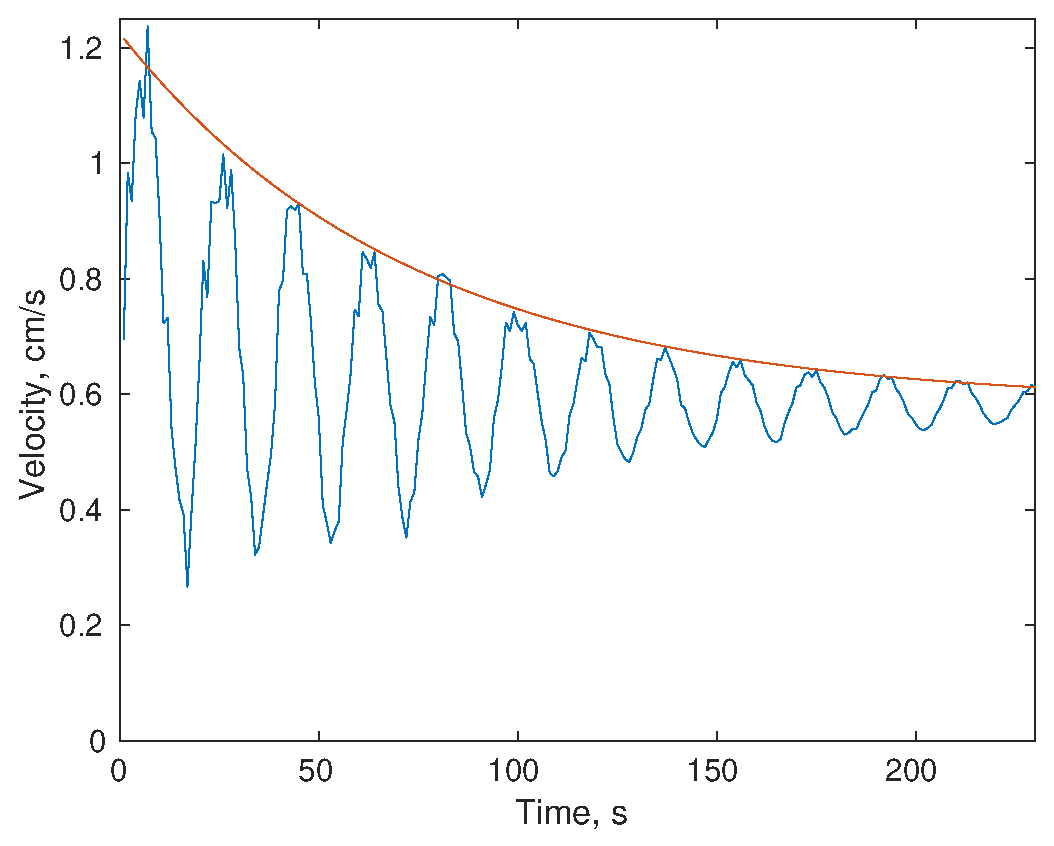
\includegraphics [width=.7\linewidth]{part6/amplVx.eps}

  \caption{Временная зависимость амплитуды горизонтальной скорости волновых колебаний. Красной кривой показана зависимость $0.58+0.60 e^{-t/75}$}
 \label{img:amplVx} 
\end{figure}

 Амплитуда этого колебания затухает экспоненциально с характерным временем около 75 секунд (красная кривая на графике показывает зависимость $0.58+0.60 e^{-t/75}$). Так образом амплитуды волны на поверхности можно приближенно описать формулой:
\begin{equation}
 \label{eq:AmplVx}
	H_x = H_0 (1+sin(\omega_0 t) e^{-t/\tau}),
\end{equation}
где $\omega \approx 0.34 \; c^{-1}$, $\tau \approx 75 \; c$.


Зная амплитуды волны можно оценить величину дрейфа Стокса, возникающего под поверхностью, по формуле \ref{eq:deepStocks}:

\begin{equation}
 \label{eq:partStocks}
	\Omega_{St} \sim H_x H_y \sim H^2_0 (1 + 2sin(\omega_0 t) e^{-t/\tau} + sin^2(\omega_0 t) e^{-2t/\tau})
\end{equation}

Усредняя по периоду $2\pi/\omega_0$ получим:

\begin{equation}
 \label{eq:partMeanStocks}
	<\Omega_{St}> \sim H^2_0 (1 + 1/2 \cdot e^{-2t/\tau})
\end{equation}

Из этих уравнений видно, что амплитуда возникающий из-за дрейфа Стокса завихренности должна испытывать колебания, причем её средняя величина будет уменьшаться с характерным временем $\tau/2$.

Таким образом, квадратичная зависимость возникающий из-за дрейфа Стокса завихренности от амплитуды волн, приводит к тому, что среднее значение завихренности должно уменьшаться со временем в течении первых нескольких минут. В то время как рисунок \ref{img:5deeps} показывает обратный эффект(среднее значения амплитуды завихренности решетки вихрей увеличивается со временем). Т.е. характер временной зависимости завихренности решетки вихрей нельзя объяснить одним лишь дрейфом Стокса. 

Обсудим влияние крупномасштабных течений на решетку вихрей.
Пространственное распределение завихренности генерируемой на поверхности жидкости определяется структурой волн. Т.е. завихренность генерируется в определенных областях пространства, после чего сносится крупномасштабным течением. Если характерная величина сноса генерируемой завихренности за характерное время установления решетки вихрей $\tau_{latt}$ будет сравнима с размером вихря $L_{latt}$, то можно говорить про существенную деформацию решетки вихрей. Таким образом можно оценить характерную скорость крупномасштабного течения, которое будет существенно сносить решетку вихрей $V_{big} \sim L_{latt}/\tau_{latt} \approx 8.5/200 \approx 0.04$ см/с. Эта оценка хорошо соотносится с средними скоростям крупномасштабных течений показанных на рисунке \ref{img:underLong} б) и в). Также из рисунков \ref{img:underLong} б) и в) видно, что при увеличении скорости крупномасштабного течения снос решетки вихрей увеличивается, что выражается в уменьшении амплитуды завихренности решетки вихрей.

Что бы ответить на вопрос как проникает решетка вихрей в объем жидкости на рисунке \ref{img:depth} показан график зависимости завихренности в промежуток времени от 500 до 600 секунд после включения накачки от глубины. Черная линия соответствует зависимости $e^{-2kh}+\sqrt{2}e^{-\sqrt{2}kh}$, где k = 0.36 см$^{-1}$, зеленая прямая - $2 \cdot 10^{-2} e^{-2kh}$. Как видно из рисунка разброс экспериментальных точек не позволяют однозначно соотнести их с одной или другой экспоненциальной зависимостью. Стоит отметить, что снос завихренности решетки вихрей из-за развития крупномасштабных течений так же уменьшает вклад решетки завихренности, продиффундировавшей из вязкого подслоя. Это в свою очередь так же может объяснять расхождение экспериментальных данных с зависимостью \ref{eq:deepEyler}.

\begin{figure}[ht]
 \center
 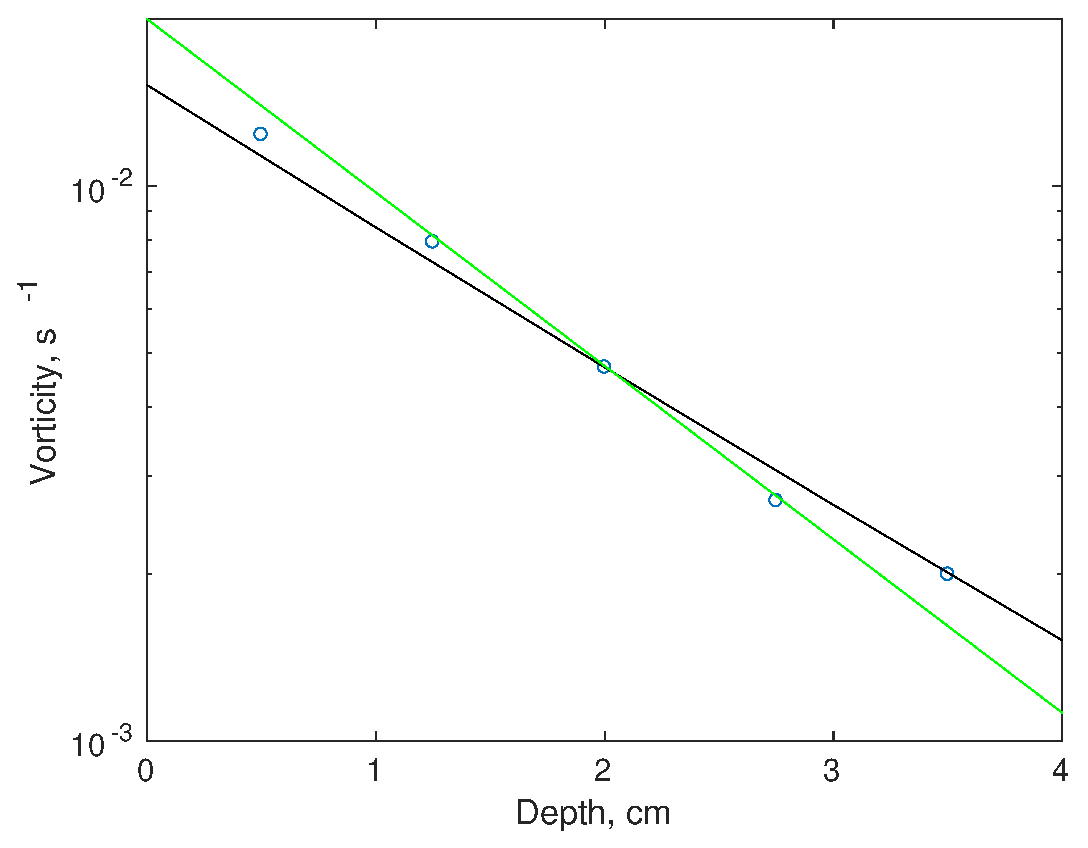
\includegraphics [width=.5\linewidth] {part6/depth.eps}
 \caption{Зависимость амплитуды завихренности решетки вихрей от глубины. Черная линия соответствует зависимости $6.3 \cdot 10^{-3} (e^{-2kh}+\sqrt{2}e^{-\sqrt{2}kh})$, зеленая прямая - $2 \cdot 10^{-2} e^{-2kh}$}
 \label{img:depth} 
\end{figure}


\section{Выводы} \label{sect6_5}
Экспериментально показано, что распределение по глубине амплитуды можно описать
%в объеме решетка вихрей структуру и зависимости амплитуды от в глубины близка к 
экспоненциальной зависимостью $e^{-2kh}$, где k — волновой вектор возбуждаемой решетки, а h — глубина слоя жидкости. 

%Экспериментально показано, что завихренность решетки вихрей под подверхностью наростает сильно медленнее, чем на поверхности воды, что свидетельствует о генерации вихревого движения в приповерхностном слое.

Экспериментально оценено характерное время $\tau \approx 200$ с проникновения завихренности решетки вихрей из вязкого подслоя в объем. Показано, что в рамках модели дрейфа Стокса нельзя объяснить увеличение амплитуды завихренности со временем.

Экспериментально показано, что наличие крупномасштабных вихрей приводит к "сносу" завихренности, проникающей в объем из вязкого подслоя. Показано, что крупномасштабные течения с характерной скоростью $5 \; 10^{-3}$ см/c приводят к существенной деградации решетки вихрей с характерным размером вихря 8 см.